program 10                                                                                                                    \documentclass{article}

\usepackage{tikz}
\usetikzlibrary{trees}

\begin{document}

% ----------- First Figure -----------

\begin{figure}[h]
\centering
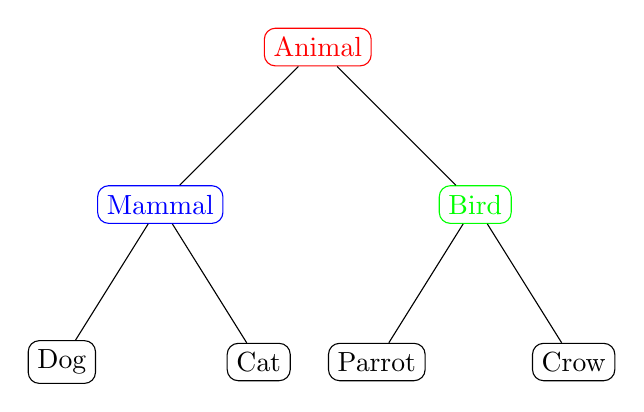
\begin{tikzpicture}[
    every node/.style={rectangle, rounded corners, draw, align=center},
    level 1/.style={sibling distance=40mm, level distance=20mm},
    level 2/.style={sibling distance=25mm, level distance=20mm}
]

\node [red] {Animal}
    child { node [blue] {Mammal}
        child { node {Dog} }
        child { node {Cat} }
    }
    child { node [green] {Bird}
        child { node {Parrot} }
        child { node {Crow} }
    };

\end{tikzpicture}
\caption{Simple Tree Diagram}
\end{figure}

\pagebreak

% ----------- Second Figure -----------

\begin{center}
\large{\textbf{Fruits}}
\end{center}

\begin{figure}[h]
\centering
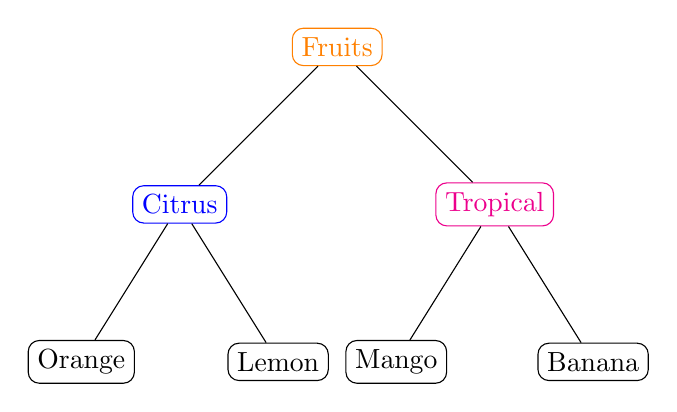
\begin{tikzpicture}[
    every node/.style={rectangle, rounded corners, draw, align=center},
    level 1/.style={sibling distance=40mm, level distance=20mm},
    level 2/.style={sibling distance=25mm, level distance=20mm}
]

\node [orange] {Fruits}
    child { node [blue] {Citrus}
        child { node {Orange} }
        child { node {Lemon} }
    }
    child { node [magenta] {Tropical}
        child { node {Mango} }
        child { node {Banana} }
    };

\end{tikzpicture}
\caption{Fruits Hierarchy}
\end{figure}

\end{document}